\clearpage
\section{Evidence across Settings and Overall Meta-analysis}\label{sec:additional_evidence}
\suppressfloats[t]

The pooled next-election association across \appMetaSettings{} settings is \appMetaEstimate{} percentage points (95\% interval \appMetaInterval{}). This appendix documents the sources, component estimates, pooling, and sensitivity. Comparisons involving longer reservation histories or survey officeholding are reported separately. Appendix~\ref{sec:additional_rural_urban} tests rural--urban differences. Differences in assignment, reservation histories, and office type limit the causal interpretation of the synthesis.

\subsection{Data sources and samples}\label{sec:additional_data}

Each comparison concerns an office in which women can hold office without a women's quota in the outcome election. The outcome is an indicator for a woman winning or being selected for that office. The exposure is prior reservation for women; the comparison group consists of offices without the corresponding prior exposure. Caste reservations may remain in either group. Conditioning on the later absence of a women's quota can select offices according to prior treatment when reservation rotates. We therefore distinguish published estimates based on an assignment design from descriptive comparisons of reservation histories.

\paragraph{Rajasthan and Uttar Pradesh.} The main electoral panels and their construction are described in Section~\ref{sec:app_data}. We retain the full-sample fixed-effects estimates for the three adjacent-election comparisons in each state for the next-election synthesis. Appendix~\ref{sec:app_additional_terms} reports the cumulative-history contrasts for the final election. The adjacent-election estimates compare reservation in the preceding election without fixing earlier histories, so they do not isolate exactly one lifetime term of exposure. Repeated elections share offices and do not constitute independent studies.

\paragraph{Mumbai.} We reproduce the 1997--2002 comparison in \citet{bhavnani2009electoral}, using the original replication data. The sample consists of \appMumbaiN{} wards with largely unchanged boundaries that were not reserved for women in 2002. The exposure is women's reservation in 1997. Wards without a treatment classification in the published comparison are excluded. Table~\ref{tab:additional_samples} reports the female-winner counts and denominators.

\paragraph{Delhi.} We link the 2007 and 2012 municipal elections using the candidate data assembled by \citet{goyal2025local}. The \href{https://sec.delhi.gov.in/sites/default/files/SEC/circulars-orders/notification-regarding-reservation-seats-2012_1.pdf}{Delhi State Election Commission's January 2012 reservation order} retained the wards established in February 2007 while assigning them to three municipal corporations. Ward identifiers therefore provide a one-to-one link for all \appDelhiLinked{} wards. We verify the earlier reservation categories against the 2007 official order and reconcile abbreviated ward names against that roster. The outcome sample contains \appDelhiOpen{} offices not reserved for women in 2012.

We use the research dataset's winner-sex field, checked against the Delhi government's municipal directory and the Association for Democratic Reforms' women-winners list. The review corrects two conflicting codes; one additional outcome has conflicting source descriptions and remains missing.\footnote{The \href{https://delhishelterboard.in/main/wp-content/uploads/2019/06/Online-Directory-2016-Delhi-Govt.pdf}{Directorate of Information and Publicity's 2016 directory} identifies the same ward and officeholder in each corrected record: Raj Kumari in ward 111 is recorded as a woman, and Mahak Singh in ward 254 as a man. The unresolved record is ward 115: the research file codes Dimple Chadha as female, whereas contemporaneous reporting uses male pronouns. We retain both possible values in the missing-outcome sensitivity.} No outcome is assigned from the ward's reservation status or from the winner's name alone.

Delhi's 2012 order assigns caste reservations by population ranking and women's reservations by alternating positions in ordered ward lists. Conditioning on a ward being open in 2012 therefore does not produce an unrestricted randomized comparison of its 2007 reservation. The Delhi estimates are descriptive.

\paragraph{Chandigarh.} We link the 2006 and 2011 municipal elections using the State Election Commission's \href{https://chandigarh.gov.in/files/documents/election-report-2011.pdf}{official election report}. The administration's October 7, 2011 letter retains the earlier 26-ward geography (PDF p.~15). The later non-quota sample contains \appChandigarhN{} wards: nine previously reserved for women and eight not previously reserved. Winner sex comes from sex-specific honorifics in the separate 2011 candidate list, linked within ward to the election results. The 2006 report includes a later by-election replacement; we retain the original general-election winner and the deferred ward-7 election belonging to that council cohort.

The October 14, 2011 directions assign women's reservations by public lottery, excluding wards previously reserved for women until rotation is complete (PDF pp.~19--20). Caste reservations follow rankings of the 2001 Scheduled Caste population share; women-reserved SC wards have a separate draw. These rules establish lottery assignment but also select the later non-quota sample. We report the conditional contrast and adjustment for prior and current caste reservation.

The \href{https://chandigarh.gov.in/files/GEMCC-2021/election-report-2016.pdf}{2016 election report} documents the same ward boundaries (PDF pp.~9--10), a fresh women's reservation draw, and updated Scheduled Caste population rankings. Seventeen wards were not reserved for women: six reserved in 2011 and eleven not reserved in 2011. We again link winner names to independently printed candidate honorifics. Four of the eleven comparison wards had been reserved in 2006; a sensitivity analysis excludes them. The two election comparisons contribute one city average to the synthesis.

\paragraph{Bengaluru.} Original State Election Commission winner gazettes and the \href{https://web.archive.org/web/20150824072502id_/http://karsec.gov.in/BBMP-2015/reservation.pdf}{2015 reservation notification} establish 198 wards under the July 2009 boundary schedule. Of \appBengaluruEligible{} wards not reserved for women in 2015, 25 were reserved in 2010 and 76 were not. We review the reservation categories against the original documents and retain the final reservation notification where it conflicts with the later winner gazette. This review corrects secondary-source women's reservation flags in two wards that affect the comparison frame.

Winner sex uses the independently recorded Gender field in the OpenCity councilor roster, checked against all winner-gazette titles. A non-sex-specific title is corroborated against the same person's title in the official ward-budget roster. Conflicting records remain unresolved, leaving \appBengaluruMissing{} missing outcome in the later non-quota sample. The statutory rotation requirement and stable boundaries do not establish a lottery for the observed assignments. We therefore interpret the Bengaluru estimates as reservation-history comparisons and examine adjustment for prior and current caste reservation.

\paragraph{Urban Uttar Pradesh.}\label{sec:up_urban}
We link the \href{https://sec.up.nic.in/}{Uttar Pradesh State Election Commission's} 2012 and 2017 municipal council and town council head-election records. Links require the same district and office type and exact body names after standardizing Unicode and spacing; ambiguous identities are excluded. The sample contains \appUpUrbanN{} offices not reserved for women in 2017, with known 2012 reservation and separately recorded winner sex. These are council heads, whereas the Mumbai, Delhi, Chandigarh, and Bengaluru samples concern ward representatives. Matching names and verified source records do not establish unchanged boundaries or random prior reservation within the later non-quota sample. We report this descriptive comparison separately from the pooled estimates.

\paragraph{Bihar.} Bihar provides a comparison of women's election as Mukhiya in 2016 according to the office's reservation in 2011. The \href{https://sec.bihar.gov.in/Documents/Panchayat_Act_Rule/ACT_Bihar%20Panchayat%20Raj%20Amendment%20Act%202009.pdf}{2009 amendment to the Bihar Panchayat Raj Act}, section 4, extended reservation to two consecutive elections beginning in 2006. Thus the 2011 exposure falls in the second election of that reservation cycle. The comparison captures withdrawal under a two-election regime; it is not a replication of the one-term municipal exposure.

We link historical State Election Commission Mukhiya winner reports to the 2016 candidate results and reservation categories within district and block. The linkage yields \appBiharLinked{} offices. Repeated identifiers are excluded, and uncertain prior categories remain missing. Among offices with known reservation in both elections, \appBiharEligible{} were not reserved for women in 2016; \appBiharN{} have an observed winner-sex outcome across \appBiharBlocks{} blocks. We recover outcomes from supplemental official winner lists only when the office is uniquely identified or the listed winner agrees with a reviewed, unambiguous vote ranking. The outcome uses explicit candidate-sex fields. Mukhiya, the village-head office, is distinct from Bihar's Sarpanch, who heads the village court.

\href{https://sec.bihar.gov.in/Documents/Panchayat_Act_Rule/RULE_Bihar%20Panchayat%20Election%20Rules%202006%20-%28%20English%29.pdf}{Rule 14 of the Bihar Panchayat Election Rules} assigns women's reservations by population ordering within reservation categories, rather than by an unrestricted lottery. Consequently, the estimates describe a selected set of reservation transitions and do not establish a causal effect of two reserved terms. The 2016--2021 pair does not provide an additional withdrawal comparison because reservation continued through that two-election cycle.

\paragraph{West Bengal appointments.} \citet[Table~III]{beaman2009powerful} report female Pradhan appointments in Birbhum, Burdwan, Hooghly, Howrah, Nadia, and South 24 Parganas. Elected council members select the Pradhan. Their sample excludes offices reserved for women in the outcome year. The 2003 regression compares offices reserved in 1998 with other offices. The 2008 regression jointly distinguishes reservation in 1998 only, 2003 only, and both years, with neither year reserved as the reference category. Regressions include district fixed effects and heteroskedasticity-robust standard errors. The six districts were selected for logistical proximity, so the results do not represent a random statewide sample. We use the published coefficients and standard errors; these are not estimates recomputed from the underlying microdata.

\paragraph{Birbhum follow-up survey.} We also analyze the reservation roster and Pradhan survey associated with \citet{beaman2009powerful}, checking the earlier reservation history against the \citet{chattopadhyay2004women} data. The roster contains \appWbRoster{} GPs; \appWbHistory{} have verified histories, of which \appWbOpen{} were not reserved for women in 2003. Sex is observed for \appWbObserved{} current Pradhans in the 2006 survey. Conflicting questionnaire fields remain missing. This measures officeholding during the term, rather than a verified 2003 appointment, and can differ if officeholders were replaced. Because Birbhum is also included in the published six-district analysis, the survey comparison is supplementary evidence on measurement and timing, not an independent replication.

\begin{table}[!htbp]
\centering
\caption{Samples for the additional microdata comparisons}
\label{tab:additional_samples}
\small
\setlength{\tabcolsep}{3pt}
\begin{tabular}{llrrrr}
\toprule
Setting & Prior quota & Eligible & Observed & Women & Women (\%) \\
\midrule
Bengaluru 2010--2015 & Not reserved & 76 & 76 & 3 & 3.9 \\
Bengaluru 2010--2015 & Reserved & 25 & 24 & 0 & 0.0 \\
Chandigarh 2006--2011 & Not reserved & 8 & 8 & 0 & 0.0 \\
Chandigarh 2006--2011 & Reserved & 9 & 9 & 1 & 11.1 \\
Chandigarh 2011--2016 & Not reserved & 11 & 11 & 0 & 0.0 \\
Chandigarh 2011--2016 & Reserved & 6 & 6 & 0 & 0.0 \\
Delhi 2007--2012 & Not reserved & 90 & 89 & 2 & 2.2 \\
Delhi 2007--2012 & Reserved & 44 & 44 & 3 & 6.8 \\
Mumbai 1997--2002 & Not reserved & 81 & 81 & 3 & 3.7 \\
Mumbai 1997--2002 & Reserved & 37 & 37 & 8 & 21.6 \\
UP urban 2012--2017 & Not reserved & 199 & 199 & 33 & 16.6 \\
UP urban 2012--2017 & Reserved & 196 & 196 & 42 & 21.4 \\
Bihar 2011--2016 & Not reserved & 534 & 527 & 72 & 13.7 \\
Bihar 2011--2016 & Reserved & 776 & 768 & 128 & 16.7 \\
Birbhum 1998--2006 & Not reserved & 69 & 66 & 11 & 16.7 \\
Birbhum 1998--2006 & Reserved & 30 & 28 & 5 & 17.9 \\
\bottomrule
\end{tabular}

\begin{minipage}{0.96\textwidth}\small
\emph{Notes:} Eligible offices have known prior reservation and are not reserved for women in the outcome election. Observed offices additionally have a resolved officeholder-sex outcome. Women's shares use observed offices as the denominator. Mumbai uses the original study's classified, largely stable-boundary wards. Chandigarh and Delhi link ward identifiers under explicit boundary-retention orders; urban UP links council heads by district, office type and body name; Bihar links 2011 and 2016 Mukhiya records. Birbhum links 1998 reservation to 2006 survey officeholding among offices open in 2003. Sources and linkage rules are described above. Published West Bengal appointment estimates lack corresponding arm-level microdata in this analysis; their regression sample sizes appear in the figures.
\end{minipage}
\end{table}
\FloatBarrier


\subsection{Next-election comparisons}\label{sec:additional_persistence_results}

Figure~\ref{fig:additional_persistence} reports the next-election estimates and their pooled summary. Rajasthan and UP retain the main analysis's full-sample fixed-effects estimates and wild cluster bootstrap intervals. For Mumbai, Delhi, Chandigarh, and Bengaluru, we calculate raw differences in proportions with Newcombe intervals combining the two Wilson score intervals \citep{newcombe1998difference}. These intervals remain nondegenerate when neither group has a woman winner. The Mumbai counts and point estimate reproduce the published comparison, while this interval differs from the original article's one-sided proportion tests. For published West Bengal estimates, we reconstruct normal intervals from the rounded robust standard errors.

Mumbai's difference is \appMumbaiEstimate{} percentage points (95\% interval \appMumbaiInterval{}), compared with \appDelhiEstimate{} points in Delhi (\appDelhiInterval{}). These are differences in female-winner probabilities among offices open to women without a women's quota, not differences in compliance with a current quota.

In Chandigarh's 2011 election, one woman won among the nine previously reserved wards, compared with none among eight previously nonreserved wards. The difference is \appChandigarhEstimate{} percentage points (95\% interval \appChandigarhInterval{}). In 2016, no woman won in either group: the difference is \appChandigarhLaterEstimate{} points (\appChandigarhLaterInterval{}). Both comparisons are imprecise.

In Bengaluru, women won \appBengaluruTreatedWomen{} of \appBengaluruTreatedN{} previously reserved wards with resolved outcomes and \appBengaluruControlWomen{} of \appBengaluruControlN{} previously nonreserved wards. The difference is \appBengaluruEstimate{} percentage points (95\% interval \appBengaluruInterval{}). These additional urban comparisons provide no evidence of a common large positive gain.

Urban UP also yields an imprecise positive difference. Women won \appUpUrbanQuotaShare{}\% of later non-quota offices previously reserved for women, compared with \appUpUrbanNonquotaShare{}\% of previously non-quota offices. The difference is \appUpUrbanEstimate{} percentage points (95\% interval \appUpUrbanInterval{}), giving each office equal weight and using a wild cluster bootstrap across \appUpUrbanDivisions{} administrative divisions. Adjustment for district, office type and prior caste reservation gives \appUpUrbanAdjusted{} points (division-clustered 95\% interval \appUpUrbanAdjustedInterval{}). Both intervals permit zero and appreciable positive differences.

Women account for \appWbBaselineEarly{}\% of Pradhan appointments in the West Bengal comparison group in 2003 and \appWbBaselineLater{}\% in 2008. Those offices were unreserved in the observed prior elections. The one-term difference in 2003 is \appWbPublishedA{} percentage points (95\% interval \appWbPublishedAInterval{}). In 2008, the recent one-term contrast, which holds 1998 reservation absent, is \appWbPublishedB{} points (\appWbPublishedBInterval{}).

\begin{figure}[!htbp]
\centering
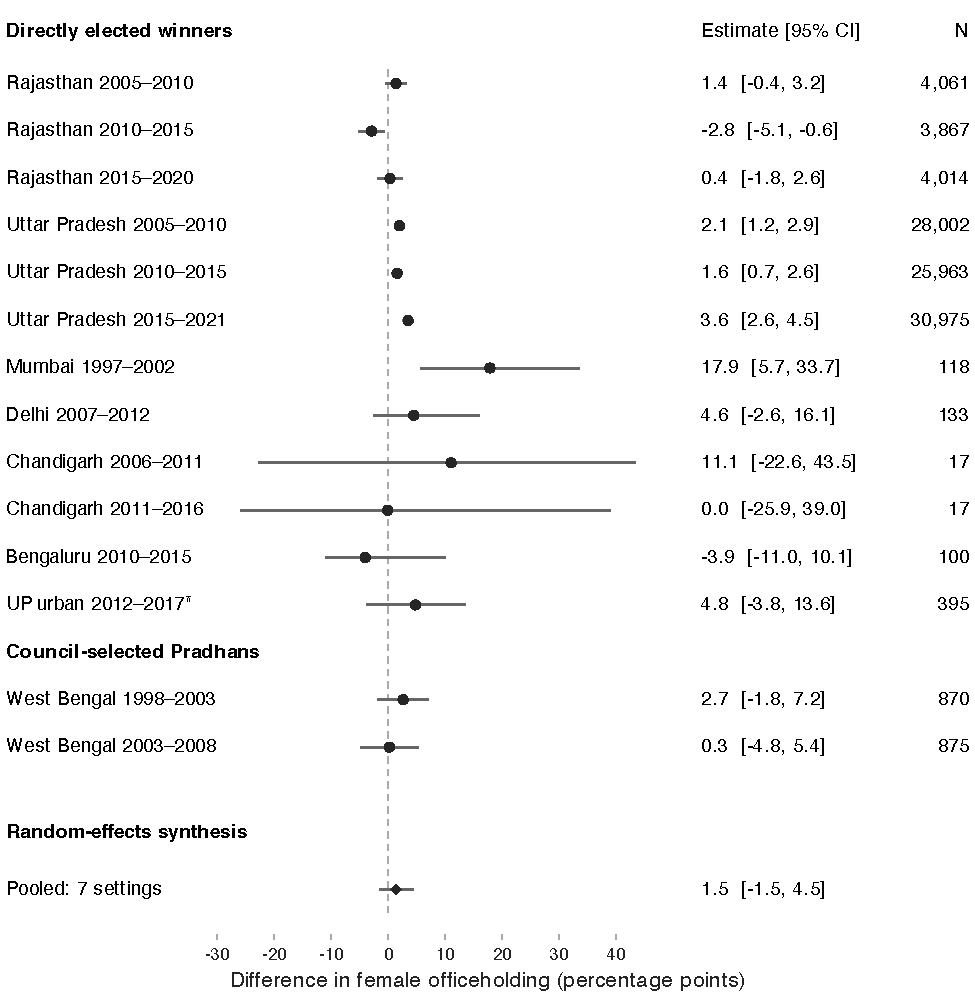
\includegraphics[width=\textwidth]{../figs/additional_persistence.pdf}
\caption{Next-election comparisons and pooled persistence estimate}
\label{fig:additional_persistence}
\begin{minipage}{0.96\textwidth}\small
\emph{Notes:} Points compare prior women-reserved and other offices among offices not reserved for women in the outcome election. Lines show 95\% intervals. Rural Rajasthan and UP use full-sample fixed-effects estimates and wild cluster bootstrap intervals; Mumbai, Delhi, Chandigarh, and Bengaluru use raw differences and Newcombe--Wilson intervals. Urban UP uses an unadjusted difference and a division-level wild cluster bootstrap with 9,999 draws. Its asterisk marks exclusion from the pooled estimate. West Bengal uses published district-adjusted estimates and normal intervals reconstructed from rounded robust standard errors \citep[Table~III, columns~1--2]{beaman2009powerful}. Its 2008 row compares 2003-only reservation with neither 1998 nor 2003 reservation. The diamond summarizes seven setting averages using Section~\ref{sec:additional_pool}. $N$ is each model's office count; overlapping samples must not be summed.
\end{minipage}
\end{figure}
\FloatBarrier

\subsection{Overall meta-analysis}\label{sec:additional_pool}

We combine the next-election comparisons in rural Rajasthan, Uttar Pradesh, and West Bengal with Mumbai, Delhi, Chandigarh, and Bengaluru. Within Rajasthan and Uttar Pradesh, we give each of the three election comparisons equal weight; within West Bengal and Chandigarh, we average two comparisons. Mumbai, Delhi, and Bengaluru each contribute one estimate. This produces one average per geographic setting, so repeated elections do not count as independent studies. Urban UP remains outside the synthesis for the reasons described in Section~\ref{sec:up_urban}. Bihar enters a sensitivity analysis because its reservation lasts for two elections. The Birbhum survey is excluded from pooling because its timing differs and it overlaps the published West Bengal sample.

The urban binary outcomes require care in estimating sampling variances. An ordinary plug-in variance is zero when both groups have no woman winner, as in Chandigarh in 2016. For every urban ward comparison, we retain the raw difference but regularize its variance: with $x$ women among $n$ offices in each arm, we use $\widetilde p=(x+1/2)/(n+1)$ and sum $\widetilde p(1-\widetilde p)/n$ across the two arms. A sensitivity analysis instead adds one to each cell. These approximate variances determine synthesis weights; they are distinct from the score intervals displayed for individual comparisons and are not guaranteed to be conservative.

The published West Bengal estimates do not report their covariance. For a common dependence sensitivity analysis across settings, we vary the assumed correlation between election estimates; a separate specification uses the estimated cross-election covariances for Rajasthan and UP from Appendix~\ref{sec:pooling}. For a setting with $m$ estimates and standard errors $s_j$, we calculate the variance of its arithmetic mean as
\[
 v(\rho)=\frac{(1-\rho)\sum_{j=1}^{m}s_j^2+\rho\left(\sum_{j=1}^{m}s_j\right)^2}{m^2}.
\]
The primary calculation sets $\rho=1$, the upper bound on the sampling variance of this mean given the marginal standard errors. These are assumptions about dependence, not estimates of it. Maximizing within-setting sampling variance does not guarantee conservative inference for the subsequent random-effects model.

We estimate the between-setting variance by restricted maximum likelihood and weight setting averages by the inverse of their sampling variance plus this estimated variance. The 95\% interval uses a modified Knapp--Hartung adjustment that cannot reduce the unadjusted standard error and a $t$ critical value with the number of settings minus one degrees of freedom \citep{viechtbauer2010metafor}. Sampling errors are assumed independent across settings. With few settings, the pooled interval and heterogeneity estimate remain sensitive to model assumptions. This exploratory synthesis covers the assembled evidence rather than a systematic sample of studies or Indian local governments.

The pooled difference is \appMetaEstimate{} percentage points (95\% interval \appMetaInterval{}), with an estimated between-setting standard deviation of \appMetaTau{} points. The average point estimate is positive, but the interval includes zero and permits both a negative association and a larger positive association.


\subsection{Sensitivity of the pooled estimate}\label{sec:additional_pool_sensitivity} Table~\ref{tab:additional_meta} varies the within-setting correlation from the primary value of one to zero, an intermediate value, and the lowest feasible equicorrelation, $-1/(m-1)$. It also adds Bihar's two-election regime, omits each setting in turn, and retains only the earliest or latest comparison per setting. Omitting West Bengal restricts the synthesis to directly elected offices. These choices alter dependence assumptions or the population of comparisons; they do not supply additional independent replications.

Alternative election weights and covariance assumptions yield similar pooled estimates (Table~\ref{tab:additional_pooling_methods}); Appendix~\ref{sec:additional_rural_urban} describes these specifications alongside the rural--urban comparison.

Omitting one setting at a time produces pooled point estimates in the range \appMetaOmitRange{} points. The primary interval includes zero, but the interval excluding Rajasthan and the interval using only the earliest comparison per setting exclude zero. The average association is therefore estimated positively, while its precision depends on geographic and temporal composition. Pooling does not resolve the selection and measurement concerns of the component comparisons.

\begin{table}[!htbp]
\centering
\caption{Sensitivity of the pooled next-election comparison}
\label{tab:additional_meta}
\footnotesize
\setlength{\tabcolsep}{3pt}
\begin{tabular}{lrrr}
\toprule
Specification & Settings & Difference & 95\% interval \\
\midrule
Primary: maximum within-setting correlation & 7 & 1.5 & [-1.5, 4.5] \\
Within-setting correlation = 0 & 7 & 1.4 & [-1.5, 4.2] \\
Within-setting correlation = 0.5 & 7 & 1.4 & [-1.5, 4.4] \\
Minimum feasible within-setting correlation & 7 & 2.2 & [-1.2, 5.7] \\
Estimated covariance in Rajasthan and UP & 7 & 1.4 & [-1.7, 4.4] \\
Urban variance correction = 1 & 7 & 1.6 & [-1.3, 4.4] \\
Include Bihar's two-election regime & 8 & 1.7 & [-0.7, 4.0] \\
Omit Rajasthan & 6 & 2.4 & [0.9, 3.8] \\
Omit Uttar Pradesh & 6 & 0.4 & [-3.2, 4.1] \\
Omit Mumbai & 6 & 1.2 & [-1.4, 3.7] \\
Omit Delhi & 6 & 1.3 & [-2.2, 4.8] \\
Omit Chandigarh & 6 & 1.4 & [-2.0, 4.9] \\
Omit Bengaluru & 6 & 1.8 & [-1.3, 4.9] \\
Omit West Bengal & 6 & 1.5 & [-2.8, 5.8] \\
Earliest comparison per setting & 7 & 2.0 & [0.8, 3.1] \\
Latest comparison per setting & 7 & 2.0 & [-1.6, 5.5] \\
\bottomrule
\end{tabular}

\begin{minipage}{0.96\textwidth}\small
\emph{Notes:} Differences and 95\% intervals are in percentage points. All rows use REML and modified Knapp--Hartung inference. Except where varied, election estimates are averaged equally within setting with correlation one. The estimated-covariance row uses the joint block-cluster covariance for Rajasthan and UP and retains correlation one for West Bengal and Chandigarh. The minimum feasible correlation is $-1/2$ for three comparisons and $-1$ for two; single-comparison settings are unchanged. Omitting West Bengal retains only directly elected offices. Including Bihar adds an eighth setting with a two-election reservation regime. Earliest and latest rows retain one comparison per setting. These are overlapping sensitivity analyses.
\end{minipage}
\end{table}
\FloatBarrier


\subsection{Other reservation histories and follow-up measures}

Figure~\ref{fig:additional_histories} presents comparisons excluded from the primary next-election synthesis because they concern different histories or outcome timing. Bihar's two-election reservation regime yields an unadjusted difference of \appBiharEstimate{} percentage points (95\% interval \appBiharInterval{}), using block-clustered HC1 standard errors and a $t$ critical value based on the number of blocks minus one.

In West Bengal, exposure in both 1998 and 2003 yields an estimated \appWbPublishedD{} percentage points at the 2008 election (95\% interval \appWbPublishedDInterval{}). That larger point estimate is imprecise and does not establish greater persistence than one reserved term. The figure also reports 1998-only exposure at the 2008 election; both contrasts use neither year reserved as the reference.

In the Birbhum survey, women hold office in \appWbControlWomen{} of \appWbControlN{} comparison GPs (\appWbControlShare{}\%) and \appWbTreatedWomen{} of \appWbTreatedN{} previously reserved GPs (\appWbTreatedShare{}\%). The unadjusted difference associated with 1998 reservation is \appWbEstimate{} percentage points (95\% interval \appWbInterval{}). This interval is too wide to establish that persistence is small. The Birbhum survey interval uses HC2 inference. Its sample overlaps the published West Bengal analysis, so it is not an independent study.

\begin{figure}[!htbp]
\centering
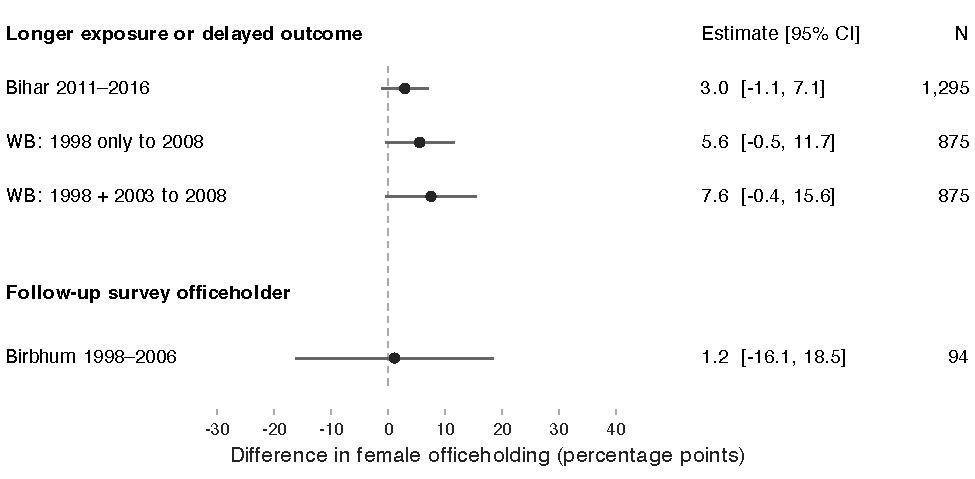
\includegraphics[width=\textwidth]{../figs/additional_histories.pdf}
\caption{Other Reservation Histories and Follow-up Officeholding}
\label{fig:additional_histories}
\begin{minipage}{0.96\textwidth}\small
\emph{Notes:} The scale matches Figure~\ref{fig:additional_persistence}. Bihar's 2011 exposure belongs to a two-election reservation regime; its unadjusted difference uses block-clustered inference. West Bengal (WB) rows compare the indicated history with neither year reserved, using published estimates and reconstructed normal intervals. Birbhum measures the current Pradhan in a 2006 survey, with an HC2 interval. All intervals are 95\%. The West Bengal comparisons share samples, and Birbhum overlaps the published West Bengal study. None of these rows enters the primary pooled estimate.
\end{minipage}
\end{figure}
\FloatBarrier

\subsection{Sensitivity to adjustment, linkage, and missing outcomes} In Delhi, assigning the unresolved outcome each possible binary value bounds the difference at \appDelhiBounds{} points over the complete eligible roster. The corresponding Bengaluru bounds are \appBengaluruBounds{} points. These are finite-roster bounds, not confidence intervals. Table~\ref{tab:additional_sensitivity} reports caste adjustments and restrictions to unchanged caste categories. We also exclude the two Bengaluru wards with conflicting primary and secondary quota codes. Such restrictions change the population being compared; restricting on later caste categories does not establish exogeneity.

In Bihar, adjustment for block fixed effects and prior caste reservation reduces the difference to \appBiharAdjusted{} points (95\% interval \appBiharAdjustedInterval{}). Restricting the linkage to exact agreement of normalized, transliterated village names produces a smaller, imprecise estimate. Name agreement establishes a narrower linkage criterion; it does not independently establish unchanged village boundaries. The \appBiharMissing{} missing outcomes bound the difference within the eligible roster at \appBiharBounds{} points. These bounds do not cover the \appBiharUnknownPrior{} linked open offices excluded for unknown prior reservation, the incomplete geographic coverage of the historical reports, or linkage errors.

In Birbhum, assigning each of the \appWbMissing{} missing outcomes both possible values bounds the difference within the verified roster at \appWbBounds{} points. Adjustment for prior caste and block, and then for current caste, also yields imprecise differences. The latter adjustment conditions on a later reservation category. These finite-roster missing-outcome bounds are not confidence intervals and do not incorporate sampling uncertainty or selection into an office being open.

\begin{table}[!htbp]
\centering
\caption{Sensitivity to adjustment and sample definition}
\label{tab:additional_sensitivity}
\footnotesize
\setlength{\tabcolsep}{3pt}
\begin{tabular}{llrrr}
\toprule
Setting & Specification & Difference & 95\% interval & $N$ \\
\midrule
Bengaluru 2010--2015 & Unadjusted & -3.9 & [-11.0, 10.1] & 100 \\
Bengaluru 2010--2015 & Prior and current caste & -3.3 & [-7.5, 0.9] & 100 \\
Bengaluru 2010--2015 & Unchanged caste category & 0.0 & [-16.8, 56.1] & 22 \\
Bengaluru 2010--2015 & Exclude conflicting quota codes & -4.1 & [-11.3, 10.0] & 98 \\
Bihar & Unadjusted & 3.0 & [-1.1, 7.1] & 1,295 \\
Bihar & Block and prior caste & 1.4 & [-3.3, 6.2] & 1,295 \\
Bihar & Name score = 1 & 1.7 & [-3.7, 7.0] & 815 \\
Bihar & Candidate results only & 3.4 & [-0.7, 7.4] & 1,289 \\
Birbhum & Unadjusted & 1.2 & [-16.1, 18.5] & 94 \\
Birbhum & Prior caste and block & 2.5 & [-18.4, 23.3] & 94 \\
Birbhum & Also current caste & 0.7 & [-20.6, 22.0] & 94 \\
Chandigarh 2006--2011 & Unadjusted & 11.1 & [-22.6, 43.5] & 17 \\
Chandigarh 2006--2011 & Prior and current caste & 13.4 & [-15.8, 42.7] & 17 \\
Chandigarh 2011--2016 & Unadjusted & 0.0 & [-25.9, 39.0] & 17 \\
Chandigarh 2011--2016 & Exclude 2006 quota exposure & 0.0 & [-35.4, 39.0] & 13 \\
Delhi 2007--2012 & Unadjusted & 4.6 & [-2.6, 16.1] & 133 \\
Delhi 2007--2012 & Prior SC and corporation & 4.5 & [-3.8, 12.7] & 133 \\
Delhi 2007--2012 & Unchanged SC category & 5.1 & [-3.9, 14.1] & 123 \\
\bottomrule
\end{tabular}

\begin{minipage}{0.96\textwidth}\small
\emph{Notes:} Differences and 95\% intervals are in percentage points. Unadjusted urban differences and the urban sample restrictions use Newcombe--Wilson intervals. Adjusted urban models and Birbhum use HC2 standard errors and residual-degrees-of-freedom $t$ intervals. Bihar clusters by district--block with the HC1 finite-sample adjustment and $t$ critical values based on the number of blocks minus one. Missing prior caste is a separate category in Bihar's adjusted model. ``Name score = 1'' requires exact agreement of normalized, transliterated village names; ``Candidate results only'' excludes recovered outcomes. The Chandigarh 2011 and Bengaluru adjustments include both prior and current caste reservation. The Chandigarh 2016 outcome is zero in every eligible ward, so adjustment cannot identify any further outcome variation. The unchanged-caste Delhi restriction and the Birbhum adjustment for current caste condition on later reservation categories. Specifications within a setting overlap and do not count as independent studies.
\end{minipage}
\end{table}
\FloatBarrier
